\begin{tikzpicture}[x=1.2cm,y=3cm,every node/.style={font=\scriptsize}]
\draw[->,gray] (-3.2,0)--(3.4,0) node[right] {$x\text{ or }\xi$};
\draw[->,gray] (0,0)--(0,1.15);
\draw[MidnightBlue,thick,domain=-3:3,samples=150] plot (\x,{exp(-4*pi*\x*\x)});
\draw[BurntOrange,thick,domain=-3:3,samples=150] plot (\x,{.5*exp(-pi*\x*\x/4)});
\node[MidnightBlue,above left] at (-.25,.9) {$e^{-4\pi x^2}$};
\node[BurntOrange,above right] at (1,.23) {$\tfrac12e^{-\pi\xi^2/4}$};
\foreach \k in {-2,-1,1,2}{\node[below] at (\k,0) {$\k$};}
\end{tikzpicture}
